\chapter{Physical Network Design}

\section{Devices}
\subsection{Workstations}
It is assumed that all workstations in use have been bought over from the old branch. The only upgrade that would have to be made to each workstation is the installation of an SFP+ network adaptor. The recommended PCI expansion card is the ASUS 10GbE SFP+ PCIe 3.0 Network Adapter.
\subsection{Wireless Access Points}
Cisco Catalyst 9136
\subsection{Layer 3 Switch}
\subsubsection{Chassis - C4506-E}
\subsubsection{Line Card - WS-X4712-SFP+E5}
\subsection{Layer 2 Switch}
\subsubsection{Chassis - C9404R}
This chassis has been chosen as it is the correct size needed to fit two supervisor cards and two line cards. Going any larger would not be beneficial and cost more. 
\subsubsection{Line Card - C9400-LC-48XS}
This line card has been chosen for the access layer switch as we can fit two of them in the chosen chassis. This will provide enough ports to cover the existing devices on each floor as well as any new devices bought in due to expansion.
\begin{table}[ht!]
    \begin{tabular}{|ccccc|}
    \hline
    \multicolumn{1}{|c|}{SKU} & \multicolumn{1}{c|}{Ports} & \multicolumn{1}{c|}{Connector} & \multicolumn{1}{c|}{Speed} & Total Needed \\ \hline
    C9400-LC-48XS             & 48                         & SFP+/SFP                       & 1/10Gbps                   & 2            \\ \hline
    \end{tabular}
\end{table}
\subsubsection{Supervisor Card - C9400-SUP-1XL-Y}
Allows for 10Gbps on each port.
\subsection{Router}
Cisco 4000 Series Integrated Services Router
\section{Wiring}
\subsection{Fibre}
A full fiber solution will be employed for this network to account for future proofing and to reduce noise on the network.
\subsubsection{Multimode Fiber - OM4}
Current network will be 10GBASE-SR, using OM4 fiber will give us options to expand to 40GBASE-SR or 100GBASE-SR in future.
Could be used in and between core/access due to high data transfer rates (10Gbps) over a distance of 550m.\\
While the distance of 550m is overkill for a 7 story building, the allowance for higher distances at higher speeds (100m at 100Gbps) will be good for future-proofing our solution.\\
Cost of fiber is reducing as time passes, basically as cheap as ethernet at this point.\\
OM4 would be used due to the cost/benefit compared to OM5 which would be overkill for our setup.\\
Will incur an additional cost of installing fiber optic enabled network cards in workstations.\\

\begin{table}[ht!]
    \centering
    \begin{tabular}{|c|c|c|}
    \hline
    Type & Distance for a 10Gbps connection & Cost per meter \\ \hline
    OM1  & 33m                              &                \\ \hline
    OM2  & 82m                              &                \\ \hline
    OM3  & 300m                             &                \\ \hline
    OM4  & 550m                             &                \\ \hline
    OM5  & 550m                             &                \\ \hline
    \end{tabular}
\end{table}

\section{Device Placement}
Change numbers of legal, marketing, finance and personnel to match google doc numbers.
\subsection{Patch Pannels}
Patch pannels could be placed on each floor to house access section L2 switches.
\subsection{Ground Floor}
\begin{figure}[ht!]
    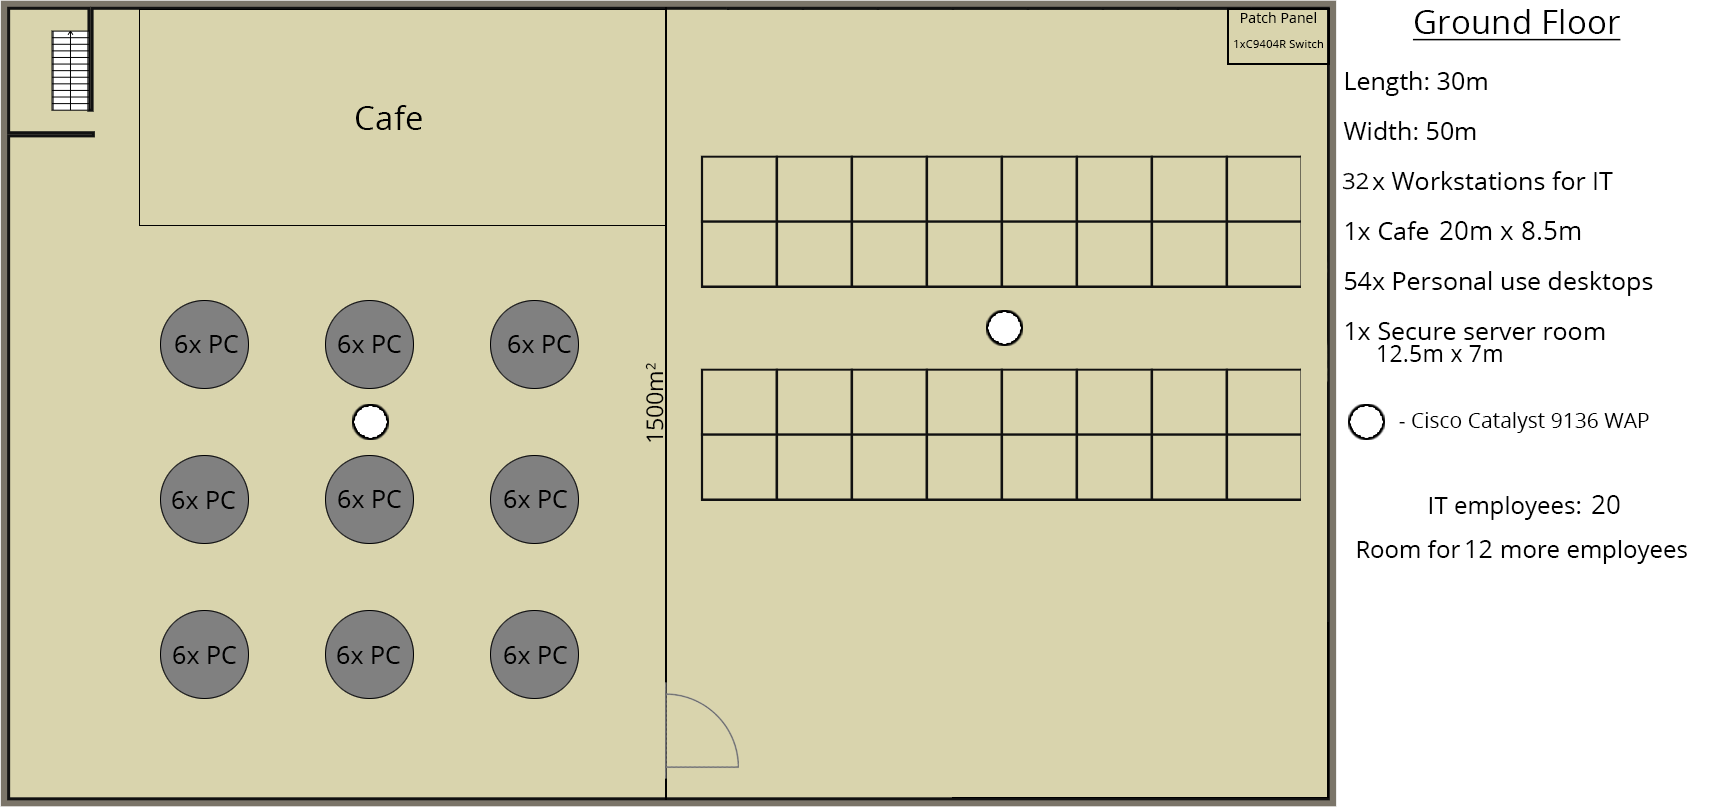
\includegraphics[width=15cm]{Figures/ground.png}
    \caption{Ground floor floor plan}
    \label{ground_floor}
\end{figure}
Change this diagram 10 to 20
\subsection{1st Floor}
\begin{huge}
    MAKE NEW 1ST FLOOR
\end{huge}
\subsection{2nd Floor}
\begin{huge}
    MAKE NEW 2ND FLOOR
\end{huge}
\subsection{3rd Floor}
\begin{figure}[h]
    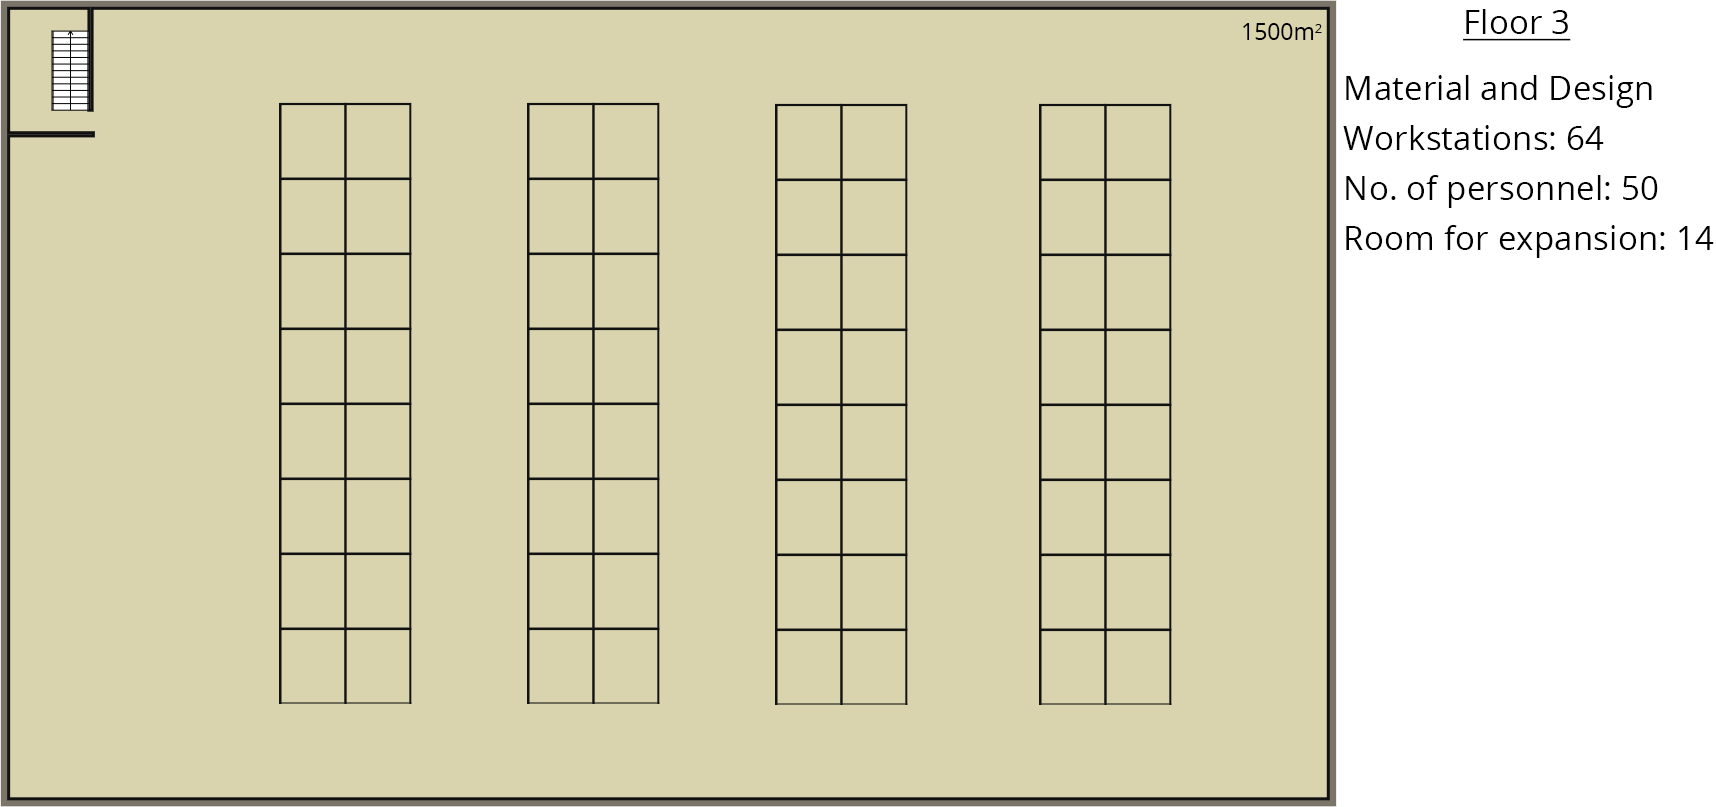
\includegraphics[width=15cm]{Figures/3rd-Floor.png}
    \caption{3rd floor floor plan}
    \label{3rd_floor}
\end{figure}
\subsection{4th Floor}
This is text
\begin{figure}[ht!]
    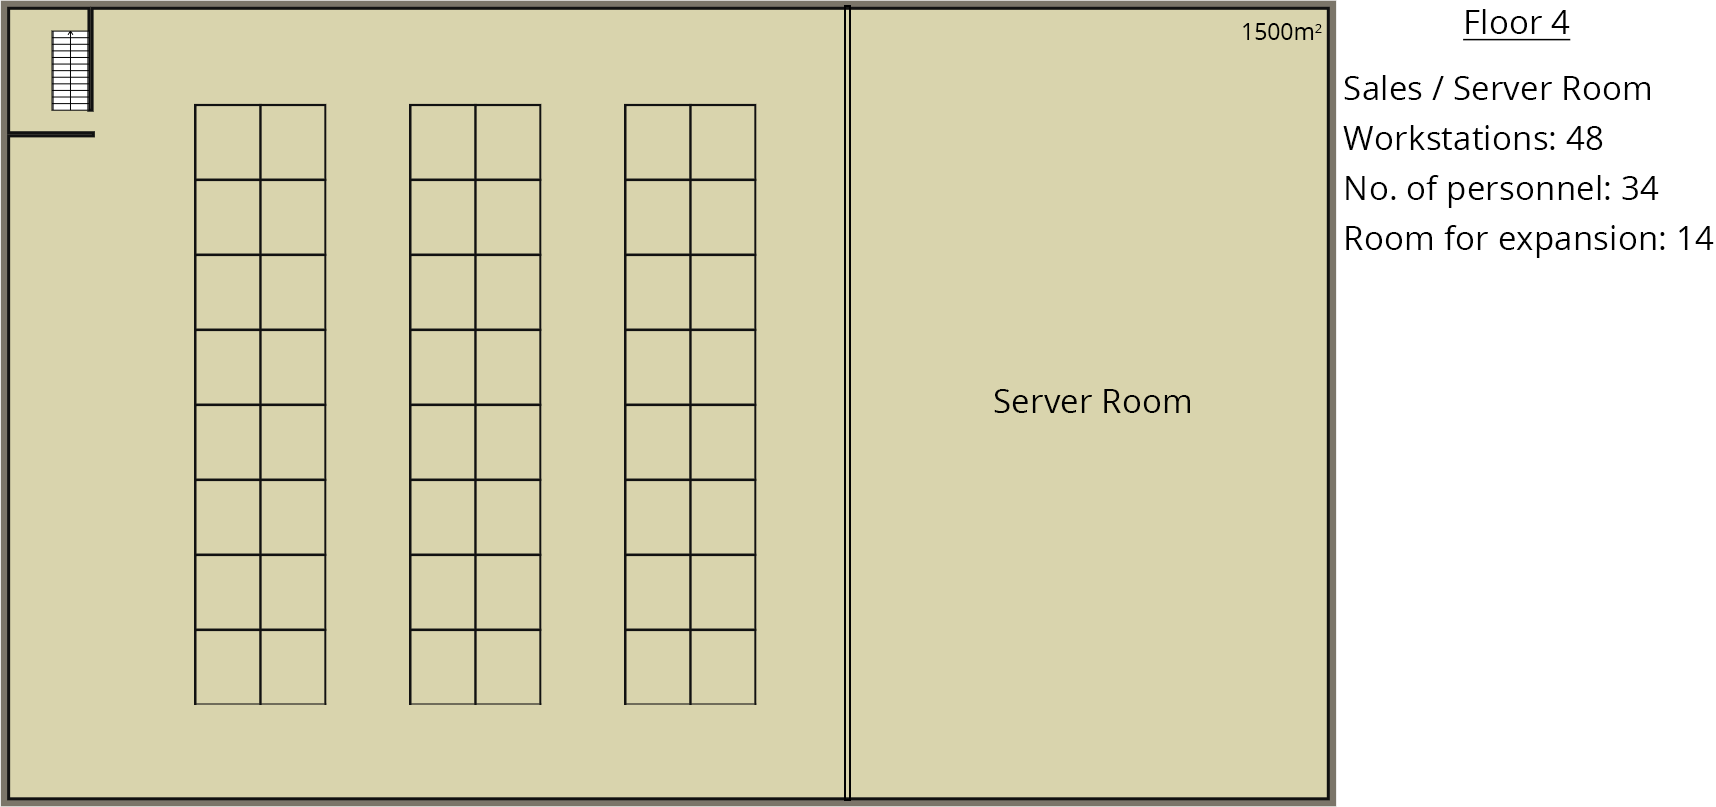
\includegraphics[width=15cm]{Figures/4th-Floor.png}
    \caption{4th floor floor plan}
    \label{4th_floor}
\end{figure}
and so is this
\subsection{5th Floor}
This is text
\begin{figure}[ht!]
    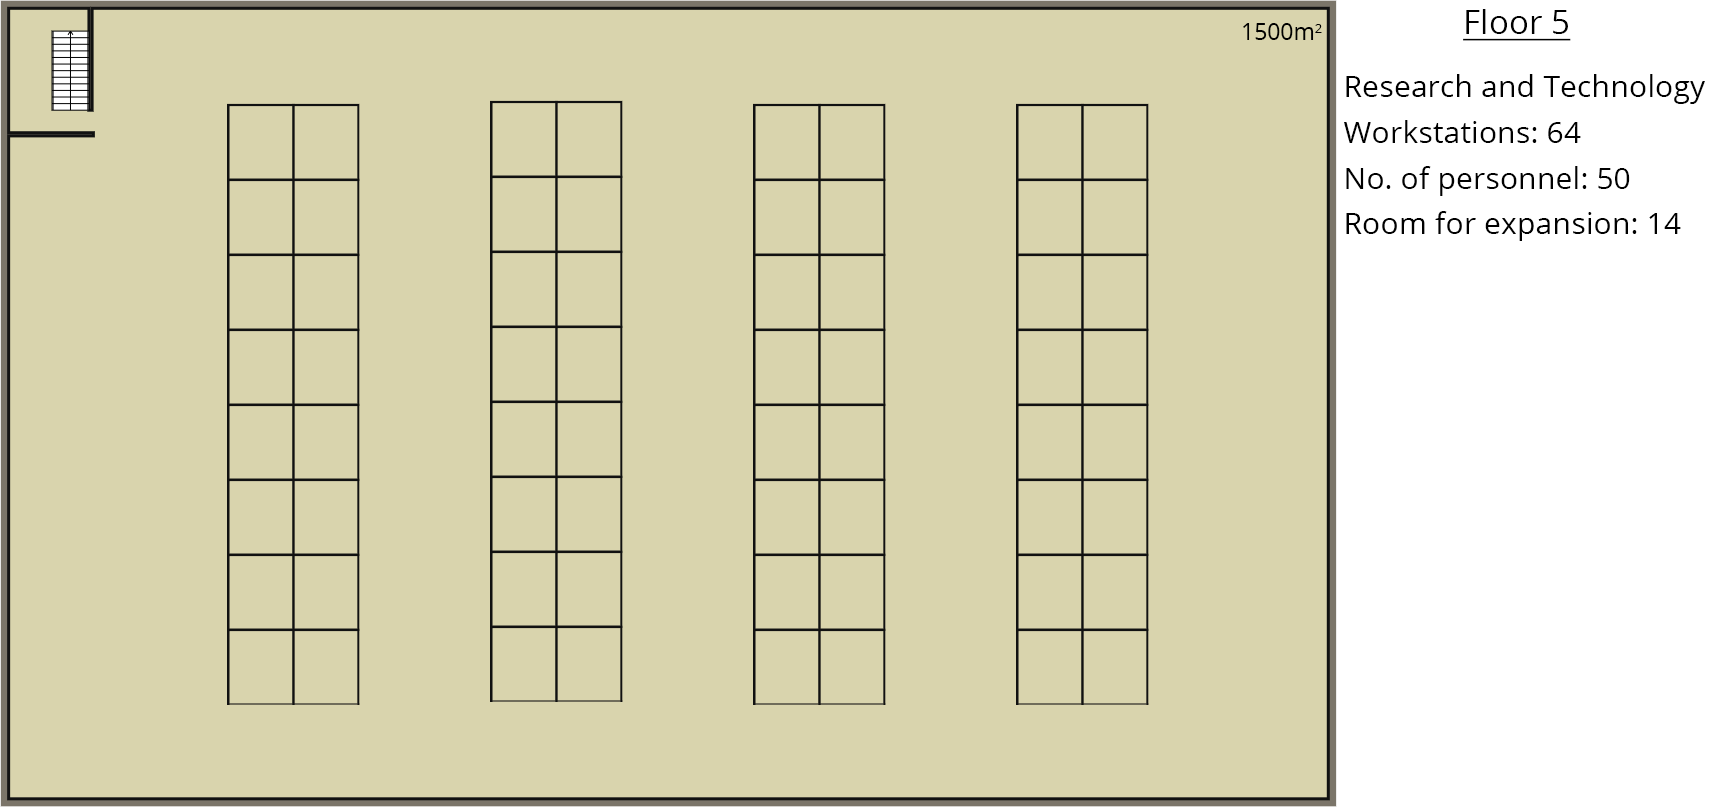
\includegraphics[width=15cm]{Figures/5th-Floor.png}
    \caption{5th floor floor plan}
    \label{5th_floor}
\end{figure}
\subsection{6th Floor}
This is text
\begin{figure}[ht!]
    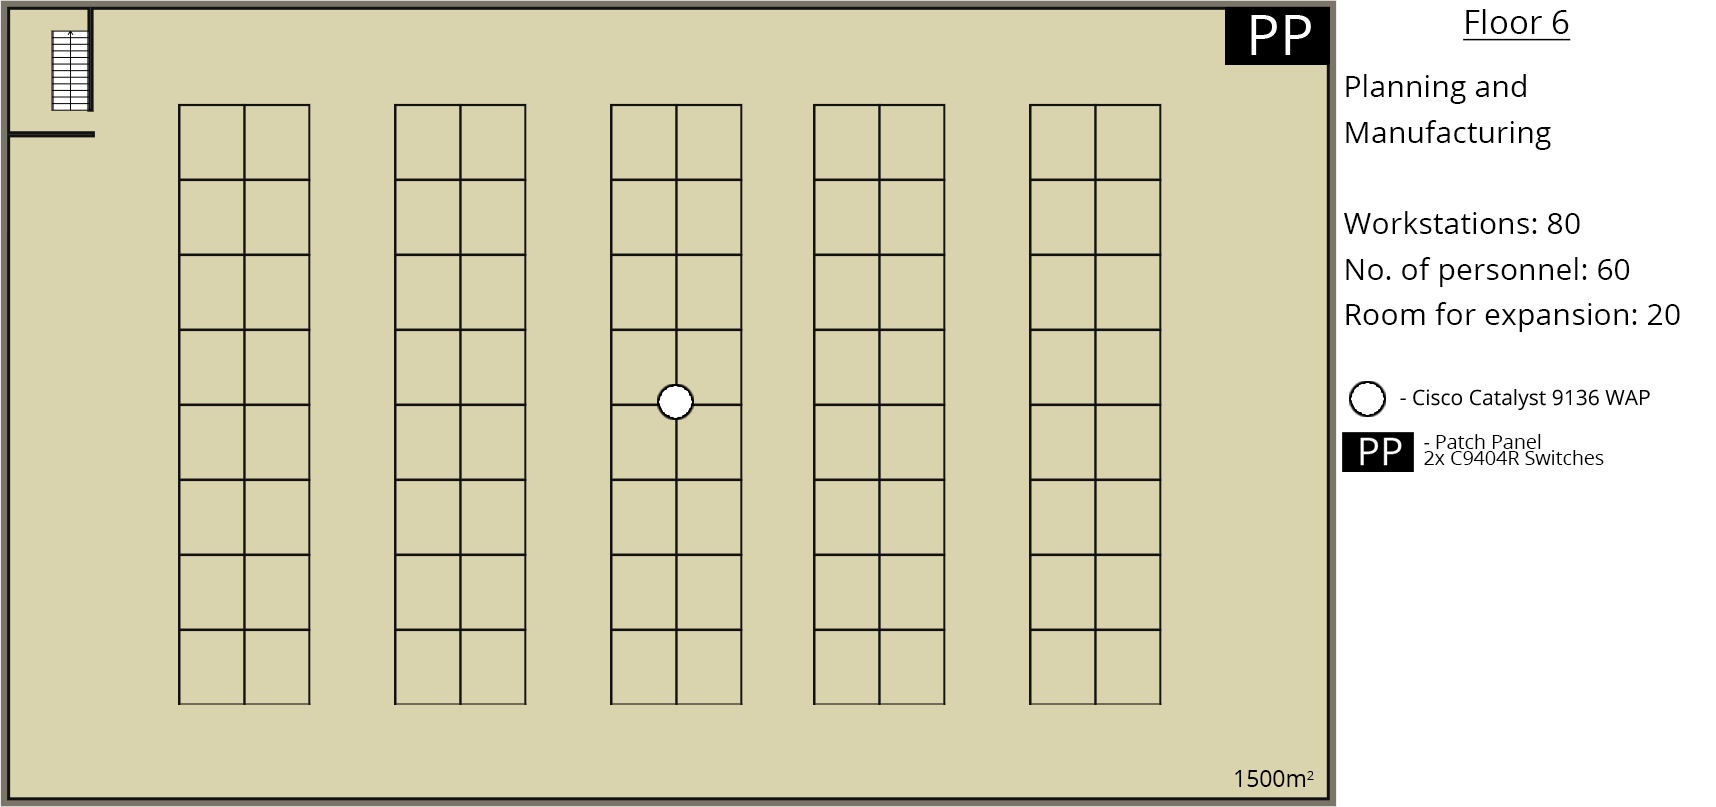
\includegraphics[width=15cm]{Figures/6th-Floor.png}
    \caption{6th floor floor plan}
    \label{6th_floor}
\end{figure}
\subsection{7th Floor}
\begin{huge}
    MAKE NEW TOP FLOOR
\end{huge}
\subsection{Server Room}